\chapter{Software Development} % application?
\label{ch:swdev}

	% Brief description and scope for this chapter	

	\section{Introduction}

	\begin{comment}
		Microestado del arte:
		Desarrollo para dispositivos android, paradigma particular, no estamos formados en él (y esto ha dado problemas), 
arquitecturas muy particulares, en el momento de comenzar el desarrollo documentación buena pero muy técnica, más para consulta que para formación. Versiones de android para usb host, … => impone requisitos al dispositivo tablet
    (Posibilidad de hilos destruidos en cada momento, atender al giro de pantalla, destrucción de la actividad, …)
    Limitaciones de android como plataforma (java vm, opengl, …)
    Aplicación iphone: funcionalidad limitada, captura de requisitos comenzó por ella, crear un producto a partir del prototipo.
    Se añadió feedback de los médicos con que trabaja Fran en Murcia (Preguntar a Recas) (en particular los logs!)

	\end{comment}

	% Introduction: app + feedback medical staff (hey, it's an important project!)
	The development of a software application targeted at Android Operating System for mobile devices is the counter-part to the hardware research part of the project.
	This application was to substitute the already developed one for iOS devices, adding funcionality extracted from feedback obtained from actual medical staff [!]Fran and EPFL[!]. The software must provide functionality to visualize ECG data from Bluetooth or 802.15.4 sources (the latter obtained via [!]our receiver node[!]) in realtime, as well as to save that data into file logs for afterwards reading.\\

	% Android general
	Android as a development platform provides a wide set of high abstraction level tools to emphasize robust and reusable design for low resource based, quick development cycles. Such benefits require the adequation of the software design and architecture to the constrains imposed by the Android development framework.\\

	% None android formation + android peculiarities
	Given that none of the project team members had received any instruction on this framework, engaging the development of an Android application implied an important risk. Moreover, after the research and training steps concluded, follow up of that risk was not halted, as the quick, robust software development is only assured when building an standard Android application; dynamic, soft real-time functionality implementation is not discouraged, but also not guaranteed to work.
	Mobile devices development restrictions and common practices were also unkown to the team.\\

	% Android limitations
	Even when the aforementioned eased development features are applicable, mobile devices are harsh software environments due to, amongst others, memory and battery constrains, where processes have to handle being suspended by an incoming call or similar external events. This factors are specially critical for an application as the one developed in this project, which needs to continually parse and log data.\\

	% App linked to hw development and a useful tool
	The application was also intended to act as a quick testing front-end for the prototypes produced by the parallel-conducted hardware research. By providing fully-functional application modules since early stages of development, hardware prototypes could be best-case and worst-case checked by directly connecting them to the Android device for data visualization. Visual verification proved to be a very effective method when working with large quantities of data which were more easily checked against their visual representation than value-by-value reading.\\

	% Development process
	These factors lead to the adoption of an agile software development process focusing on functionality building while prototyping more high risk involving features. To avoid typical drawbacks of such methodologies, great emphasis was put on the application of characteristics found in \textit{Iterative and Incremental processes}, namely, use case driven and risk focused development. That way, project scheduling was done addressing higher risks first while assuring expected functionality to be implemented on time thanks to the use case model.\\

	\section{Overview}
	% Conclusion and chapter presentation
	In the following sections a complete view of the software development project will be presented, beginning with the requirements captured for the project. The use case scenarios identified from those requisites will be detailed next, followed by an explanation of the system architecture ?via 4+1 view model?. Then implementation details will be exposed and the chapter will finish with a short conclusion.

	\begin{comment}
	Full implementation, architectural and yadda yadda are presented in Annex X
	\end{comment}

	\section{Requirements}
		% Requirement capture process explanation (also introduction to this section)
		The requirement capture process for the project considered three main stake-holders: the project masters (¿Nombres?), the EPFL[*] and the project team members; and was done in two sessions. The first one produced the basic requirement list which described the system and was used to schedule the earlier development iterations. This was so because of the strong time restrictions this software development project had to cope with. 
		When the critical functionality was achieved and the hardware research was in a suitable state, the second requirements capture session was conducted. By then, the +EPFL representative (Fran) [Murcia Hospital representative?] had shown the state of the development to the stakeholder party of him, and collected feedback. Thus, the requirements produced by this second session were of a more user-oriented nature.\\

		% ¿Explicar qué intereses tiene cada uno?
		
		% Y ahora, esto:
		The functional and non-functional requirement lists are presented next.

		\subsection{Functional Requirements}
		\begin{itemize}
		\item R01 - Receive raw data via Bluetooth
		\item R02 - Receive raw data via 802.15.4
		\item R03 - Receive raw data from a log file
		\item R04 - Parse raw data into processed data
		\item R05 - Display processed data
		\item R06 - Log raw data
		\item R07 - Log processed data	% Delete if not developed
		\item R08 - Scale View Vertically
		\item R09 - Scroll View Vertically
		\item R10 - Scroll View Horizontally
		\end{itemize}

	% ?Non-functional requirements?
	% 30fps
	% USB-host Android 3.1

		\subsection{Non-functional Requirements}

		The following non-functional requirements are identified:
		\begin{itemize}
			\item The application must display ECG data at 30fps.
			\item The application must run on a Motorla Xoom device.
		\end{itemize}

	\section{Risk Analysis}

		Being the project mainly a hardware research project, and considering the software development part of it useless without successful results on the hardware part, a detailed process of risk analysis was mandatory to be conducted since the earlier stages of planning and development so as to avoid wasting manpower on futile work.\\

		The risk list at the end of the project is as follows:
		\begin{itemize}
		\item \textbf{PR1.} Application funcionality inferior to that featured by existing iOS application

		\item \textbf{HR1.} 802.15.4 receiver device delayed
		\item \textbf{HR2.} 802.15.4 receiver device unfeasible

		\item \textbf{MR1.} Mobile device unsuitable for target functionality

		\item \textbf{AR1.} Lack of instruction on Android development delays workflow
		\item \textbf{AR2.} Android providing subpar performance when handling required data
		\item \textbf{AR3.} Android rendering capabilities unable to handle required data
		\end{itemize}

		% Risk anaylisis process explanation (decisions, ...)
		This risk anaylisis focused on two main risk sources: the parallel-conducted hardware research, and Android as a development platform. Project definition and team related risks were also considered.\\

		The hardware research part of the project delivered the highest probability and impact rated risks. It was so because those risks were external to the software development project scope and thus could not be handled by any of the tools provided by any development methodology. At the same time, should such risks come to be, the impact on the software product would be, in most of cases, as cathastrophic as turning the whole development useless thus causing it's cancellation.\\
		
		Regarding Android development only a subset of the final set of risks was assessed at first. Every risk in this subset dealt with the team lack of knowledge about the Android platform and was scheduled to be addressed foremost. A last risk was added to this group after the first research on mobile devices limitations regarding potential unfitness of such devices for near real-time display and handling of not-so-small data packages, and that risk handling plan proved to be key to the successful outcome of the project as the remaining subset of Android-related risks were linked to Android applications display performance.\\ % Further explanation on this last set?

		The usual project definition and personal risks such as incorrect deadline scheduling or unability to reach critical milestones on time were pondered, increasing their impact rates as the application would be needed by the hardware device to secure a successful outcome for the project.\\
		
		% Risk Table including evolution
		A detailed view of each assessed risk is provided next, including risk evolution throughout the project lifetime.\\

		% PR1
		\paragraph{PR1.}Application functionality inferior to that featured by existing iOS application\\
		\textbf{Probability:} Moderate\\
		\textbf{Impact:} Very High\\
		\textbf{Description:} Failure to provide an expanded set of features in the Android application when compared with the iOS application renders the software part of the project invalid on its own. It could, then, only be valid as demo software for USB receiver device showcasing. If the device is nor finished, then the whole software development project will have been futile.
		The key marker for this risk is unability to generate valid software modules throughout the development that provide required functionality. Failure to reach milestones and use case realizations on time is other important marker.
		Preventive measures were taken to avoid the occurence of this risk since the beginning of the development by a functionality building focused project scheduling for the first development phases.\\
		\textbf{This risk was marked as surpassed at the reviewing metting of Iteration 2 as all key functionality had been implemented, as planned.}

		% HR1
		\paragraph{HR1.}802.15.4 receiver device delayed\\
		\textbf{Probability:} High\\
		\textbf{Impact:} High\\
		\textbf{Description:} Being the production of the 802.15.4 receiver device dependant on the hardware research part of the project a delay on the estimated milestones for that part of the project is likely to occur. Should that happen, hardware research and development will need to be prioritized over this software project. That could lead to big delays in software production.
		To prevent the rising of further problems derived from those potential delays, the software development process must always work with non-solid, ready-to-change deadlines and milestones. Application functionality is to be ranked in order of importance of implementation to be prepared, in case of an unexpectedly big delay, to leave less important functionality out of the scope of the project.
		Markers to be followed up are: unsuccessful output from hardware research (a new branch of the potential technologies tree has to be explored), failure to reach hardware development or research milestones and delays in the acquisition of tools or devices needed for the hardware project.
		Preventive measures considered are: detailed follow up of the hardware research development, reducing the software development team if manpower is needed in the hardware area, and planning asuming delays on component acquisition.\\
		\textbf{HR1 was monitored throughout the whole software development project, and marked as surpassed at the reviewing meeting of Iteration 5.}

		% HR2
		\paragraph{HR2.}802.15.4 receiver device unfeasibe\\
		\textbf{Probability:} Medium\\
		\textbf{Impact:} Critical\\
		\textbf{Description:} Until hardware research results are successfully delivered there is no guarantee of the viability of the 802.15.4 receiver device. This software development project loses most of its value if such device is not developed, as the iOS application already exists. Developing an Android application with an equal feature set is also a valid objective, so this risk does not render the development invalid: the full team will then work on software development, and requirements will be restated to include more final-user oriented functionality and/or features from the \emph{future} set.
		This risk can be monitored with the following markers: unsuccessful output from hardware research and failure to reach hardware development or research milestones. Being both external to this software project, no preventive measures can be applied apart from scheduling allowing smaller team sizes for the software area.\\
		\textbf{The probability of the risk was reduced to low after the reviewing meeting for Iteration 3, when the critical hardware research had concluded with positive results. HR2 was marked as surpassed when the production of a device prototype was finished and tested [?TIME?].}

		% MR1
		\paragraph{MR1.}Mobile device unsuitable for target functionality\\
		\textbf{Probability:} Low\\
		\textbf{Impact:} Critical\\
		\textbf{Description:}Even when mobile devices technical specifications have increased significantly in the previous years, specially regarding CPU power and rendering capabilities, the soft-realtime requirements of the project in terms of data manipulation and visual representation involve a low probability risk of the application being unsuitable for such devices. The risk probability is decreased by the fact that similar featured applications exist both for iOS and Android powered devices. Even so, the 802.15.4 receiver device USB interface doesn't allow for this risk not to be reckoned.
		Preventive measures considered: quick prototyping of critical functionality to discard  unfeasibility, conduction of performance tests, both rendering and data handling related, in the target device and testing of USB-Android communication as soon as possible in the project schedule.\\
		\textbf{As performance tests were conducted on early builds of the application, the need of further research on this risk arised as the data handling performance in the target device was low, but not as low as the rendering performance. Thus, this risk was unfolded into risks AR2 and AR3, both related to Android performance when handling the aforementioned tasks. This risk follow up was then halted, as it was no longer needed.}

		% AR1
		\paragraph{AR1.}Lack of instruction on Android development delays workflow\\
		\textbf{Probability:} High\\
		\textbf{Impact:} Moderate\\
		\textbf{Description:} None of the team members has received any instruction on Android development and throughout research is not viable because of time restrictions. It is reasonable to foresee potential delays in the development because of the parallel instruction-development flow, as well as the need to rewrite parts of the system rendered obsolete when further knowledge is acquired.
		Application malfunctioning, unexpected behaviours and low performance are markers to be tracked.
		As a preventive measure a short instruction time will be scheduled at the beginning of the project, but every team member is responsible to continue his instruction throughout the whole project. Application builds are to be checked for big differences against canon Android applications behaviour.\\
		\textbf{The risk was marked as surpassed after Iteration 3, as critical functionality had already been implemented and tested, though Android instruction was not halted.}

		% AR2
		\paragraph{AR2.}Android providing subpar performance when handling required data\\
		\textbf{Probability:} Moderate\\
		\textbf{Impact:} High\\
		\textbf{Description:} The benefits of the high-level, single application model provided by Android are such in behalf of the sacrifice of performance. In this project soft-realtime requirements are present, and the system needs to process around 250 ECG wave samples [quotation needed] (among other data) per second. Android code reutilization and class based programming suggested practices, the absence of an explicit memory management API and the employment of the Garbage Collector only complicate the achievement of such requirements.  
		Special care will need to be put on the development and performance checks are to be conducted regularly on generated builds to ensure the avoidance of this risk.
		If evidence is found of Android inability to provide the required perfomance (and there is no way of attributting the failure to the team's lack of ability), low-level Android development will be considered. As the probability of this last scenario to occur is quite low, no research will be conducted in low-level Android development until mandatory.\\
		\textbf{The risk was verified to be occuring during Iteration 2 testing phase. Lack of care on memory management was found to be the problem, and was solved in Iteration 3. The risk was marked as surpassed after the review meeting for Iteration 4.}

		% AR3
		\paragraph{AR3.}Android rendering capabilities unable to handle required data\\
		\textbf{Probability:} Low\\
		\textbf{Impact:} High\\
		\textbf{Description:} The Android Operating System runs on quite a wide range of devices, each with its own technical specifications. Providing the single application development model that Android features requires many software layers, many of them of high abstaction level. The risk exists, thus, that the rendering required by the project couldn't be achieved within the involved time restrictions. The target device for the project is fixed (see Non-functional Requirements Subsection [link!]) as a Motorola Xoom. This device employs a dedicated Tegra2 GPU [quotation needed] which should suffice, so risk probability is chosen as \emph{low}. Performance tests in the display module are to be conducted, though, so as to make sure that a correct usage of the available resources is being done. 
		If low rendering performance is detected, Android native level rendering API, Renderscript, is to be looked into as a remedy, once the code is assured to be optimized.
		\\
		\textbf{Risk probability was increased to \emph{Moderate} during Iteration 3 as low performance was detected but was considered not critical enough to apply the Renderscript solution. The risk was marked as surpassed in the reviewing meeting of Iteration 4.}\\

		% Conclusion
		Thanks to this risk analysis the project schedule was developed in such a manner that it prioritized risk suppressing and the decision was taken to plan only the first two of the five intended development iterations, leaving the other three as drafts to allow them to evolve at par with the uncancelled risks.
		Use case realization order was also selected based on this risk analyisis, ensuring that higher risk involving features were developed (or at least prototyped) as early as possible.\\
		
		Use cases for the project are presented next, followed by the system architecture description, to allow a finer understanding of the software development project schedule and related decissions, which will be detailed in the next section.
	
% Command to auto-generate Use Case headings (NON FUNCTIONAL YET)
\begin{comment}
\newcounter{uccounter}
\newcommand{\addUC}[1]{
	\stepcounter{uccounter}
	\bf{UC\arabic{uccounter} #1}
	}
\end{comment}
	
	\section{Use Cases}

		The project use cases are now presented following the \emph{use case common style} described by Martin Fowler [Fowler, 2004], as the relaxed template allows for quicker document producing than more detailed descriptions such as those presented by Cockburn [Cockburn, 2001].\\

		Actor listing is omitted in all the descriptions, because of the following implicits:
		\begin{itemize}
			\item The main actor for the use case is the user
			\item The only other actor is the data emitter node, when applicable. It can refer to the Bluetooth emmitter device or the USB 802.15.4 receiver device.
		\end{itemize}
		Please note that the 802.15.4 emitter node is not considered an actor as the communication with such device is handled by the USB 802.15.4 receiver, which actually is the considered actor.

		\subsection{UC1. View data from Bluetooth}

			\paragraph{Description} The user wish to receive and visualize data from a Bluetooth ECG node in real time. He will start the communication, visualize real-time received data and finish the connection once done.\\
			\\This use case captures requisites R01, R04, R05, R06, and R07.

			\paragraph{Preconditions} The application is in the main menu screen.
			\paragraph{Main flow}
				\begin{enumerate}
				\item User indicates his will to start Bluetooth data visualization.
				\item The system prompts for the node to connect to.
				\item User specifies the desired node.
				\item The system manages connection to the node. If unable to establish the connection, see AF1.
				\item The Bluetooth node sends data to the system.
				\item The system shows processed data to the user. Received data is also logged.
				\item The user can now adjust view parameters (See UC4)
				\item User chooses to finish data visualization.
				\item The system closes active connections and stops data visualization.
				\item The system returns to the main menu.
				\end{enumerate}

			\paragraph{Alternative Flow 1} The system cannot establish connection to the Bluetooth node selected by the user.
				\begin{enumerate}
				\item The system notifies the user about the problem.
				\item The system returns to the main menu.
				\end{enumerate}

		\subsection{UC2. View data from USB Receiver}

			\paragraph{Description} The user wish to receive and visualize data from 	an 802.15.4 ECG node in real time. He will start the communication, visualize real-time received data and finish the connection once done. The data from the node will be received via the USB 802.15.4 receiver device.\\
			\\This use case captures requisites R02, R04, R05, R06, and R07.

			\paragraph{Preconditions} The application is in the main menu screen.
			\paragraph{Main flow}
				\begin{enumerate}
				\item User indicates his will to start USB receiver data visualization.
				\item The system asks the user to connect the USB receiver.
				\item User connects the USB receiver.
				\item The system manages connection to the USB receiver. If unable to establish the connection, see AF1.
				\item The USB receiver device sends data to the system.
				\item The system shows processed data to the user. Received data is also logged.
				\item User can now adjust view parameters (See UC4)
				\item User chooses to finish data visualization.
				\item The system closes active connections and stops data visualization.
				\item The system returns to the main menu.
				\end{enumerate}

			\paragraph{Alternative Flow 1} The system cannot establish connection to the USB receiver device.
				\begin{enumerate}
				\item The system notifies the user about the problem.
				\item The system returns to the main menu.
				\end{enumerate}

		\subsection{UC3. View data from log file}

			\paragraph{Description} The user wishes to read a log file created from a real time visualization session. He will specify the log file to load, visualize stored data and finish visualization once done.\\
			\\This use case captures requisites R03, R04 and R05.

			\paragraph{Preconditions} The application is in the main menu screen.
			\paragraph{Main flow}
				\begin{enumerate}
				\item User indicates his will to start log data visualization.
				\item The system prompts for the log file to load.
				\item User specifies the desired file.
				\item The system reads the selected log file.
				\item The system shows logged data to the user.
				\item User can now adjust view parameters (See UC4)
				\item User chooses to finish data visualization.
				\item The system stops data visualization.
				\item The system returns to the file selection menu.
				\item User selects to return to main menu. Else follow from step 3.
				\item The system returns to the main menu.
				\end{enumerate}

		\subsection{UC4. Adjust view parameters}

			\paragraph{Description} When visualizing ECG data the user wishes to adjust view parameters such as plot vertical scale, plot vertical scroll and plot horizontal scroll.\\
			\\This use case captures requisites R08, R09, R10.

			\paragraph{Preconditions} The application is displaying ECG data.
			\paragraph{Main flow}
				\begin{enumerate}
				\item User indicates his will to change the vertical scale.
				\item The system updates plot vertical scale.
				\item User indicates his will to change plot vertical scroll.
				\item The system updates plot vertical scroll.
				\item If the displayed data is read from a log file, see AF1.
				\end{enumerate}
			
			\paragraph{Alternate Flow 1} The user is able to control horizontal scroll parameter.	
				\begin{enumerate}
				\item User indicates his will to change the horizontal scroll.
				\item The system updates plot horizontal scroll.
				\end{enumerate}

	\section{Design and Architecture}

		\begin{comment}
		Design made targeting easy expansion of the code.
		Android development framework imposes the utilization of a derivate of the Activity class as the entry point for the application. The idea is that an application is composed of various Activities, providing each of them a screen with which users can interact in order to do something \todo{Cite Android Dev Guide}. 
		\end{comment}

		The design of the software application is done targeting easy extension of the functionality which allows an incremental realization of the identified use cases and quick, isolated prototyping of new features in a manner in which already developed ones are not afected.\\

		The Android Software Development Kit being the base technology employed in the development, the Android Application Framework conditions the basic architecture of the system. Particularly this framework imposes the utilization of a derivate of the Activity class as the entry point for the application. The idea is that an application is composed of various Activities, providing each of them ``a screen with which users can interact in order to do something'' \todo{Cite Android Dev Guide}.\\

		The correct usage of the activities model in the Android framework includes declaration of them in the application manifest (see X \todo{Actually reference something} for reference) and a number of other steps which are excessively formal for the target comfort and speed-of-operation levels regarding development of extensions. Specifically the application gives support for a number of data sources, namely Bluetooth, log file and USB device, each one with it's own needs in terms of user interfaces and interaction. Moreover, new data sources would possibly require different interfaces than those already developed.\\

		In such an scenario the decision is made for the architecture of the application to override Android activities model, employing only a single Activity which will implement a stack of user interfaces each with its own logic and behaviour, in the same manner Android does with the activities but allowing more flexible development. The inclusion of a new interface or set of interfaces is, thus, simplified, and every application entity is given the ability to present it's own menu to the user. This is specially useful when including new data sources with special interface requirements to the application.\\

		An overview of the application architecture is presented in \autoref{fig:arch-global}.\todo{Explain here the package division (Activity + View + Data + Model Realizations) and place image?}

		\begin{figure}[h]
		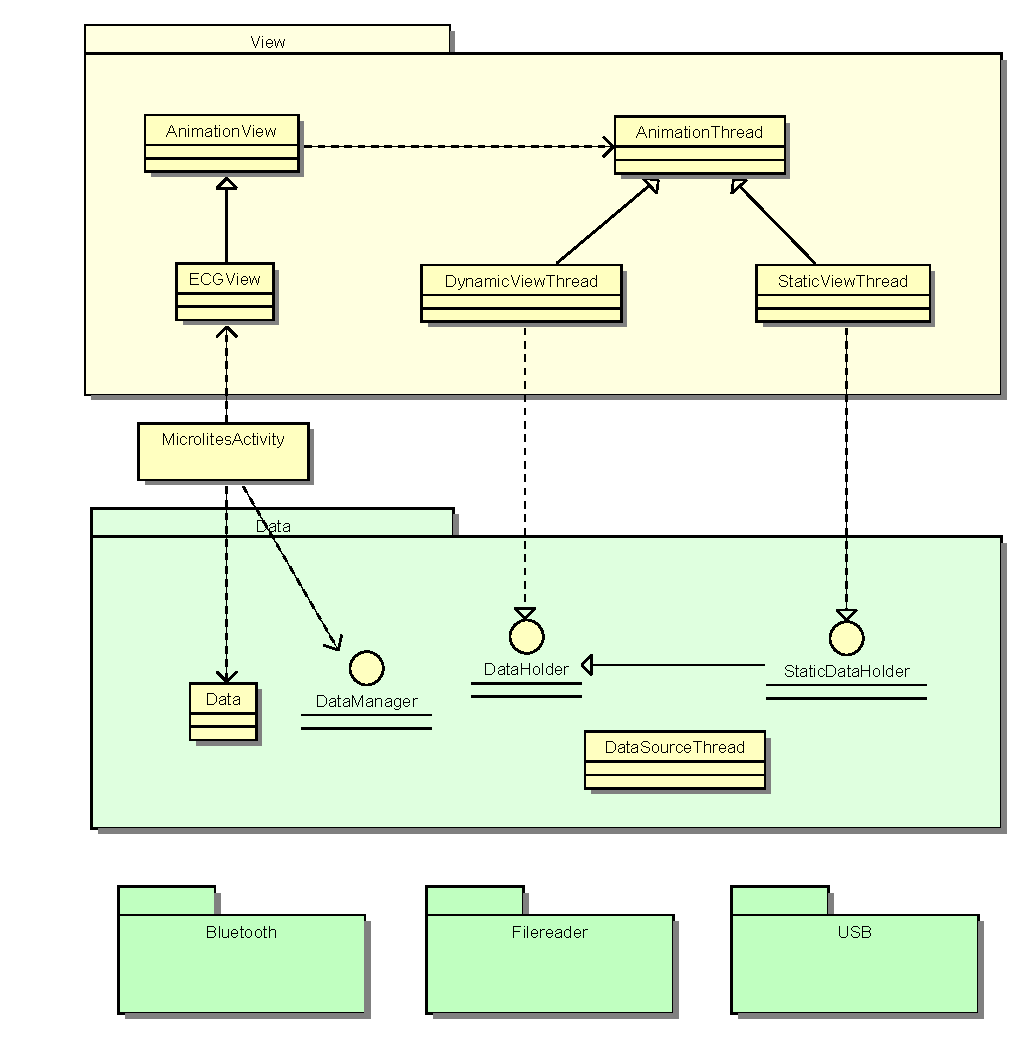
\includegraphics[scale=0.5]{mlts-arch-main}
		\centering
		\caption{Architecture overview}
		\label{fig:arch-global}
		\end{figure}

		At the core level the main Activity, the View package and the Data package are present, as well as three packages (Bluetooth, Filereader, USB) which will be dealt with later. These components provide the basic elements which compose the model over which actual functionality is built, and are to be seen as the tools available for the overlaying software layer which is addressed next.\\

		The main Activity of the application assumes the role of the central coordinator and is responsible for creation and management of area specific managers, application level data and handling of the aforementioned user interfaces stack. It is also responsible, as the application's entry point, of the presentation and behaviour management of the main application menu which gives access to actual functionality, delegating in the specific managers.\\
		
		Of all those tasks, the most important are the initialization and eventual finalization of data visualization flows in collaboration with the appropiate area specific manager. Throughout the process, mainly controlled by the activity, components required for the visualization process are initialized, delegating area specific tasks to the manager. Eventually, the manager assumes the control of the application flow, leaving the activity as a dispatcher of input events.\\

		% Model: Core, domain specific components that require realization in order to work.
		% Model involves: a Manager, a DataSource and a DataHolder (as well as a DataParser) and, if visualization is required, the ECGView and a ViewThread derivate.
		% The model needs to be realized for it to work, the Activity is just an engine running an instance of the model.
		% "It follows a factory pattern, but the factory is the Activity."

		These managers are part of the so-called, in the project terminology, a model; and the activity can be portrayed as the model manager. Conceptually a model is a set of software entities which live in the application and handle the data flow from a given data source towards a data holder, including or not, the visualization of such data. A model contains a Manager which is the entity responsible of the handling of the rest of the model entities. Please note that this model scheme is  specific to the domain of the project and is not a general one\todo{Remove this note? Leave this note?}.

		\begin{figure}[h]
		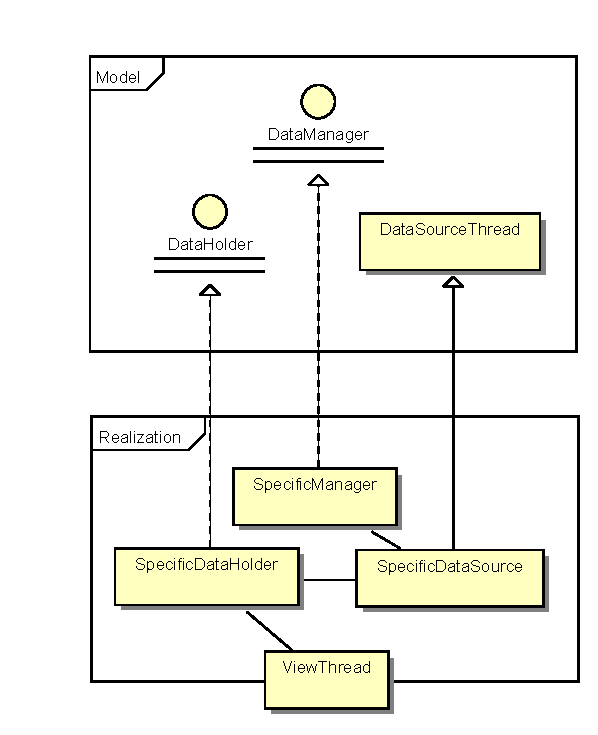
\includegraphics[scale = 0.5]{mlts-arch-model}
		\centering
		\caption{Data-flow model realization}
		\label{fig:arch-model}
		\end{figure}

		This conceptual model \todo{Rename model to FlowModel?} scheme is provided by a subset of the classes and interfaces shown in \autoref{fig:arch-global}. For actual functionality building a realization of the model is to be developed, giving actual meaning to the scheme. In the scope of the project four model realizations have been implemented and will be detailed later.\\

		A model realization is composed of implementations of the following elements from the core level exposed before: 1) a Manager, which handles user interaction and required preparations; 2) a DataSource that manages raw data obtention from the actual source, and processing and sending of such data to a 3) DataHolder, which stores and handles the data in any required way and, if data visualization is required 4) an implementation of a view thread.\\

		More detailed approaches to all the concepts exposed in this introduction are built throughout the following subsections.

		\subsection{View Package}
		\begin{comment}
		Realtime rendering required a special, non full common functionality (slide, scroll, ...) providing View derivate: SurfaceView. It provides a bitmap surface where you can draw whatever you want. Derived into AnimationView with employment of AnimationThread for obtaning a good old while(!finished) \{update(); render();\} loop.
		That structure derivates into ECGView which is a domain specific specialization of AnimationVeiw and Dynamic- and StaticViewThread. The later two implement behaviour expected of Dynamic and Static data visualization respectively (more on this on the Data Package)
		Programming style in this area closer to C than to an OOP language in order to maximize performance. (Talk about intolerable initial performance caused by extreme number of new each step and too much relaying on GarbageCollector?)
		\end{comment}

		The set of classes encompassed in the View package (see \autoref{fig:arch-global}) provides both a base rendering architecture in an update-render loop style not initally present in the Android framework and the specialization of such architecture for the specific project domain, i.e. plotting of the electrocardiogram wave and it's relevant points.\\

		The soft real-time rendering imposed by the project restrictions requires a special, non common functionality providing Android View \todo{reference to View in andev?} class derivate: the SurfaceView. This kind of View provides a bitmap surface where pixel-level rendering is allowed. A set of rendering tools is also provided by Android. The architecture developed on top of that view extends the SurfaceView to an AnimationView and delegates the rendering to an AnimationThread. This last entity is the one providing the update-render loop employed for the real-time rendering.\\

		The actual, domain specific rendering functionality providing threads are implemented employing the aforementioned layer as a base. The precise entities are DynamicViewThread and StaticViewThread, and are referred in this document as implementations of the view thread, even if such class does not exist in the project. This two classes implement the required behaviour for dynamic and static data visualization respectively, and obtain the data to be shown from a data source entity. Such entity is dealt with in the following section. The reason for different entities to exist for static and dynamic rendering is also developed there.\\

		\subsection{Data Management Package}
		\begin{comment}
		Data class acting as a centralized data storage. Provides app-level syncronization too.
		Different models for static and dynamic data management.
		Dynamic: manages its own data and implements replacemente and discard politics, data is provided by single units. This is so because of the way the data is received and then parsed in real-time.
		Static: obtains a reference to the data location, which is where the actual data manipulation is done. This way huge ammounts of data transfering is avoided (read file can contain lots of megabytes of data which can't be passed at once to the holder). First try was passing the whole array of samples but that was unassumable in real-time.
		DataSourceThread is a receiver by concept, but concrete implementations might require actual communication, that is, data reception \emph{and} data sending. As a developer facility, any DataSourceThread must provide an implementation of a method for writing data into the actual raw data source, expected to act in a similar manner to the one the DataSourceThread does in the inside.
		\end{comment}
		
		This package contains data storage and handling related entities. Differentiation between two types of data managed by the application depending on their purpose is mandatory. On one hand is the application level data, which is specific or non-specific information shared by the whole application. On the other hand is the data received from a source that must be visually presented to the user or stored for later visualization. Providing software tools allowing the modelling that data flow is the key task of this package.\\

		The class Data acts as a centralized application level data storage. It is a singleton and is accesible by every entity in the system. It also provides syncronization methods for correct inter-thread communication.\\

		The rest of the entities of the Data package are employed in the aforementioned model scheme, and specify the expected behaviour of each element involved in a data flow. As indicated before, specialization of this entities is required for the realization of the model.\\

		DataManager is the interface to be implemented by the model controller. It is responsible for the configuring, starting and halting the data flow provided by its controlled entities. It also participates in the process of initialization of the visualization \todo{Link to this process} of a data flow by communicating a DataHolder with the respective DataSourceThread.\\

		A DataSourceThread is a thread which provides data to other entities in the system, generally to a DataHolder. It is a specialization of Thread with functionality to start and stop the flow of data. This data is usually received from an external entity, such as a USB device or a file, and concrete implementations  might require an actual communication between the two, forcing the DataSourceThread to send data to the other end of the connection. Because of that, any specialization of this class must also listen to petitions of writing to it's data provider when available.\\

		The processing of raw data sent by the data providers to the DataSourceThreads is expected to be done in the latter, so the data transfered throughout the application is of a processed nature. To this end the DataParser entity is available\todo{Reference DataParser}.\\

		The expected receiver of the data sent by a DataSourceThread is a DataHolder. This interface provides domain-specific data handling abstract methods and definitions. An implementation of a DataHolder must handle the reception of ECG wave samples, delineation points, synchronization points and heart-beat-rate values.\\

		The actual way in which that data is employed depends on the concretion of the interface, and might or might not involve visual representation. When visual representation is required, the view thread implementation should also implement the DataHolder interface.\\

		%Dynamic: manages its own data and implements replacemente and discard politics, data is provided by single units. This is so because of the way the data is received and then parsed in real-time.
		%Static: obtains a reference to the data location, which is where the actual data manipulation is done. This way huge ammounts of data transfering is avoided (read file can contain lots of megabytes of data which can't be passed at once to the holder). First try was passing the whole array of samples but that was unassumable in real-time.

		There are two different specifications for the data holders: DataHolder and StaticDataHolder. This is so because of the two modes of operation\todo{Is it clear that there are two modes of operation?} of the application. One is real-time data visualization and the other is log file visualization. The former is called dynamic visualization and the latter static visualization, and the behaviour of their DataHolders is not the same.\\

		Dynamic visualization represents data received in realtime by the DataSourceThread. The DataSourceThread obtains the data from an external entity, processes it and sends it to the DataHolder. This data usually arrives in groups of variable size, and is provided to the DataHolder in single units once processed. In this scenario the DataHolder is the view thread, and handles data however considers is the optimal way. In the implementations developed in this project a fixed ammount of data is held and older information is replaced by the new one as it arrives.\\

		Static visualization, on the other hand, involves reading a file, usually megabyte sized. The receiving of big quantities of data in single units by the data holder, as would occur if  the original DataSource specification was employed, could lead to severe slow-downs and application performance would be affected. To avoid such issues, the StaticDataHolder specification is developed.\\

		A StaticDataHolder doesn't actually hold the data: it delegates that task to it's DataSourceThread. The data source will provide the StaticDataHolder with a reference to the actual data. This way big ammounts of data transferring is avoided. The inheritance relation between DataHolder and StaticDataHolder is imposed by the architecture, which require a DataHolder to be passed to a DataSourceThread.\\

		\subsection{Utilities Package}
		\begin{comment}
		Contains application level reusable components as two different DataParsers (one for realtime, on for static data which doesn't store what it reads). Also contains the Viewport entity employed as a container of the view parameters. An unused color picker is there (not mention!)
		\end{comment}
		This package contains reusable components providing very specific functionality so they are considered utilities: RealTimeDataParser, StaticDataParser and Viewport.\\

		A data parser is the entity responsible of the processing of the raw data obtained by a DataSource into the domain specific data that the application manages. There are two implementations, one for real-time data reception, RealTimeDataParser, and the other for static data reading, i.e. a log file. The real-time data parser is also responsible of storing the received raw data the a log file.\\

		A data parser is intended to be contained in a DataSourceThread. It receives the bytes of raw data and, upon successful identification of a valid data element, notifies the corresponding DataHolder entity of the arrival. In a theoric, performance-independant model, this behaviour would be incorrect: the data parser would leave the processed data \emph{in} the DataSourceThread, which would then make the transfer of information to the data holder. This kind of implementation is not valid with the soft realtime requirements of the project, as the data source - data parser - data source - data holder flow would be a severe bottle-neck.\\
		
		\subsection{Realization of the Model 1: Bluetooth}
			BluetoothManager handles bluetooth connection, launches two different threads one of them being the DataSourceThread implementation, the former being a non-blocking connection starting thread.
			Employs a DynamicViewThread which implements DataHolder interface and receives data from Bluetooth's ConnectedThread.
			This ConnectedThread holds the DataParser and provides de data directly to DVT.

		\subsection{Realization of the Model 2: FileReader}
			FileManager handles the selection of a file by the user (previous presentation of available ones), creates file reading thread providing the chosen file and connects this with the viewthread.
			FileDataSourceThread is at the same time a DataSource and a DataHolder. Because of that, it doesn't realize the DataSource interface. This is an example of the flexibility sought by the design: were mandatory to have implemented the DataSource interface, another stage in the data flow would have been added, slowing things up (even if only because of synchronization mechanisms)
			Employs an StaticViewThread which doesn't hold data and gets references to the actual data location in FileDataSourceThread when needed. 
			FileDataSourceThread, thus, manages data reading and holding, and manipulation. Explanation follows: data is read from files with the aid of a FileConverter entity (explain?). This files can be of big size, so they shouldn't be fully load onto memory. A partial load is mandatory in such cases, and the next chunk of data is to be read when the "visualization window" approaches. All that management is done by the FileDataSourceThread. When the view is controlled (scroll horizontal) the event is passed directly into this thread from the ViewThread (which receives the input from Activity). FileDataSourceThread updates the pointers to the visualized data start and end (can do because it works on time rather than on pixel units [3 seconds to be seen onscreen == 750 data samples]) and passes them to viewthread as well as the rest of the data. That way, if more file reading is required, it can be done in a transparent-to view manner.

		\subsection{Realization of the Model 3: USB}
			DeviceManager handles device enumeration and selection. As there's only as much as one available usb device (at the time) no selection is needed, when the device is detected, connection is done, but it can easily be implemented.
			USBComThread is the DataSourceThread realization, which, given the endpoints of the usb connection to a device, handles data reception from the read endpoint, parses it and sends to its DataHolder, which is a DynamicViewThread. As cannon as it gets, baby.

		\subsection{More things (which I don't know where to include}
			
			\texttt{(These with sequence diagrams and all)}
			Explanation of the visualization initialization procedure, as well as the finalization one.
			Example of a full data flow (e.g. bluetooth)

	\section{Implementation Details}

		\begin{comment}
			Potential iterations
			It1. Bluetooth + Architecture prototype
			It2. USB + Log
			It3. Architecture rewriting
			It4. Adding it all and finishing

			For iteration description:
				+ objectives
				+ objectives description
					realization, done?
				+ Use Cases realized
				+ expected and spent time
				+ extra objectives
				+ prologue to next iteration

			Describe risk statuses updates in each iteration?
		\end{comment}

		% Intro
		In this section a detailed description of the development is presented. The evolution of the application architecture and functionality; design, architectural and implementation decisions and explanations of the circumstances in which they were made, as well as the development of the project schedule are exposed in chronological order.\\

		The section is arranged following the five iterations of the project, developing each one by presenting the target objectives and expected deadlines for the iteration, detailing application evolution with emphasis on use case realization and risk suppressing achievements and demonstrating the state of the project as assessed on the reviewing meeting conducted at the end of the iteration.

		% Scheduling
		\subsection{Project Scheduling}
			
			Before diving into the description of the development process an overview of the project schedule % and the reasons for it to be as open as it is
			is mandatory.\\

			As was mentioned in the previous sections, an agile software development methodology has been applied to the project, even if artifacts from more ordered and structured methodologies have been employed to avoid losing focus on the critical aspects of the development.\\
	
			Software development project being dependant on parallel-conducted hardware research, project assets, both personal and development resources, being shared with the hardware research having the former higher priority, and team's lack of formation regarding Android development are some of the factors which lead to the adoption of such a mixed methodology. As they have been already exposed in previous sections, they won't be detailed here.\\ %Consult [X][Y][Z]... for details

			In such an scenario, a fully developed, eight month covering schedule was unfeasible, at least with the imposed time restrictions which didn't allow much time to be spent on planning. The decision was then made to plan only the earlier project iterations, assuring critical functionality identified from use case development to be implemented as soon as possible as well as higher threat involving risk suppression to be realized.\\

			Actual software project development begun October 15, 2011, being the final deadline set on June 15, 2012. That deadline could not be pushed any further, so an estimated deadline was set on May 31, 2012, leaving half a month for further work or recovering from delays, and seven and a half months of development time.\\
		
			Time was needed for the hardware research to start providing results, and no work could be done in the meantime on related application parts. Considering also that even in the most optimistic scenarios no actual work with the 802.15.4 USB receiver couldn't be done until mid February [link to hw planning or something], the schedule had to assume that the first four months of software development would need to cover the implementation of most of the features, leaving the rest of the development time for implementing hardware-related requirements, which couldn't actually be scheduled until hardware research was evaluated.\\

			The adopted schedule dealt with the aforementioned facts by proposing five iterations, from October 15 to May 30, complying with the fifteen days reserved for contingencies. The first three iterations had a duration of two months, the third one a single month, and the remaining one was fifteen days long.\\

			Having the previously developed iOS application as starting point, and being achieving at least the same feature list of that a critical target of the project, the first two iterations were planned so as to realize \textbf{UC1} and \textbf{UC3} which captured requisites expressing such feature list.\\

			The next iterations were just scrapped as no accurate estimation could be done on the state of the project by those dates. Thus, the third iteration was planned to cover the implementation of the remaining features, namely, communication with the 802.15.4 receiver device, the fourth one reserved for polishing the application and the fifth one left for testing and validation. The fourth iteration was to shrink if objectives were achieved quickly to leave more time for validation.\\

			The scheduled distribution of work for each iteration is as follows:\\

			\begin{tabular}{| c | l | l |} % | l | para el hw
				\hline
				It & Dates & Activity \\ \hline
				1 & Oct 15 - Dec 15 & Application base and Bluetooth module\\ \hline
				2 & Dec 15 - Feb 15 & Log module and initial USB module\\ \hline
				3 & Feb 15 - Apr 15 & Final USB implementation \\ \hline
				4 & Apr 15 - May 15 & Polishing \\ \hline
				5 & May 15 - May 30 & Validation \\ \hline
				- & May 30 - Jun 15 & Reserved \\
				\hline
			\end{tabular}\\\\

			Which can be seen as the following expected use case realization dates:\\

			\begin{tabular}{| c | l | l |} % | l | para el hw
				\hline
				It & Dates & Realized Use Case \\ \hline
				1 & Oct 15 - Dec 15 & UC1, UC4 (first version)\\ \hline
				2 & Dec 15 - Feb 15 & UC3, UC2 (first version)\\ \hline
				3 & Feb 15 - Apr 15 & UC2 (final) \\ \hline
				4 & Apr 15 - May 15 & UC4 (final) \\ \hline
				5 & May 15 - May 30 & Validation \\ \hline
				- & May 30 - Jun 15 & Reserved \\
				\hline
			\end{tabular}\\\\

			Throughout the development, as expected, this schedule had to be adapted as the hardware research advanced to assess the arise of difficulties and subsequent changes to its planning. Instead of providing a fixed snapshot of the altered schedule at the end of the project, a detailed description of each iteration is presented next, including modifications to the planning and the motivation for making them.

		\subsection{Iteration 1}

			The main objectives for this first iteration were
			\begin{itemize} 
				\item the instruction of the team on Android development, 
				\item the lay out of an initial version of the application architecture and
				\item the implementation of the Bluetooth receiver module.
			\end{itemize}

			The alloted time for the iteration was of two monts, from October 15 to December 15. During this period the hardware research didn't require much resources [link to hw], so in practical terms the full team was employed in the software project.\\

			In order to minimize risk AR1[quote?link?], the instruction of the team on Android development becomes the key objective for the iteration. Development starts with the implementation of the designed base architecture for the application, so it serves as a powerful learning resource. The notion of that implementation as disposable is not abandoned throughout iteration time and it is always considered as a prototype to evolve or be substituted by a more refined version once team's knowledge of Android increases.\\

			Having the basic architectural framework developed, implementation of the Bluetooth receiver module begins. Special care is put both on design and implementation, as this functionality has to be ready as soon as posible, and little time will be available for reimplementation further in the development.\\

			Testing of both architecture and Bluetooth module is conducted during the whole iteration, specially in the final weeks, so by the end of the iteration Bluetooth module is validated and expected to be stable until the scheduled architectural redesign.\\

			As the Android formation phase takes less time than expected and hardware research doesn't allow advancing into next iteration at the time iteration objectives are achieved, an extra implementation effort is put to begin implementation of UC4. Adjust View Parameters.\\

			In the review meeting for the iteration the following conclusions are obtained:
			\begin{itemize}
				\item Basic architecture implementation is done.
				\item Android is confirmed to be a very comfortable development environment even if non-standard functionality is not that easily achieved. Instruction is planned to continue.
				\item Realization of UC1-View data from Bluetooth is finished. Related user interface is not final, but it is functional, and is to be updated on further iterations.
				\item Realization of UC4-Adjust view parameters is done in relation to Bluetooth visualization. As remaining modules are developed, further work is to be done in this field.
			\end{itemize}

			\begin{comment}
			Results and adaptation of pre-planned it2
			Risk evolution!?
			\end{comment}
			
		\subsection{Iteration 2}

			The main objectives for the second iteration were
			\begin{itemize} 
				\item the development of the USB communication module and
				\item the implementation of the Log visualization module.
			\end{itemize}

			Log writing improved.
			USB module done as USB device, valid for arduino and first msp tests
			Log reading implemented, scrolling and such. Tests results indicate low performance, huge memory requirements.
			With the basic interface, first Prototype with (except usb host == 802.15.4) full functionality implemented. That nice and all. Shown to masters and feedback applied.
			On time ?

			Took a loong break here for hardware development
			% Here ends electroiltes

		\subsection{Iteration 3}
			% This is microlites
			This is the first just-drafted iteration. Starting from the fully functional prototype, architectural and performance fixes were mandatory. Also, given the positive state of the hw research scheduling was done for the rest of the iterations.

			The main objectives for this third iteration were
			\begin{itemize} 
				\item the redesign of the application architecture, 
				\item the achievement of required performance in data management and
				\item the scheduling of the rest of the project time.
			\end{itemize}

			~(Scheduling seems strange as an objective)~

			Architecture redesigned targeting easy adaptation and versatility inside the scope of the application. Redesigned visualization initialization flow.
			Performance increased significantly and memory usage reduced THROUGHOUTLY in realtime view.
			Fixes in modules according to new architecture.
			Talk about scheduling??

		\subsection{Iteration 4}
			Final implementation iteration. Final performance increasing fixes and user interface implementation, as well as user-friendliness globally increased.

			USB Host here!

			The main objectives for this third iteration were
			\begin{itemize} 
				\item the implementation of USB host communication,
				\item the achievement of required performance in rendering and, 
				\item the implementation of user-friendly interfaces.
			\end{itemize}

			This ends the implementation phase, user-friendlyness could be better but what gives. 
			Performance left 50-50 because it was already ok (30fps not 60fps).
			One iteration left, devoted to testing.

		\subsection{Iteration 5}
			Testing and validation with the real thing.

			Hey, us of the future, I hope everything's ok up there!
			
	\section{Closure}
